%%%%%%%%%%%%%%%%%%%%%%%%%%%%%%%%%%%%%%%%%
% Beamer Presentation
% LaTeX Template
% Version 1.0 (10/11/12)
%
% This template has been downloaded from:
% http://www.LaTeXTemplates.com
%
% License:
% CC BY-NC-SA 3.0 (http://creativecommons.org/licenses/by-nc-sa/3.0/)
% Colaboración:Edison Abado Ancco
% 145012 - UNSAAC - INgeniería electrónica
%
%%%%%%%%%%%%%%%%%%%%%%%%%%%%%%%%%%%%%%%%%

%----------------------------------------------------------------------------------------
%	PACKAGES AND THEMES
%----------------------------------------------------------------------------------------
%
%\documentclass{beamer}
\documentclass[aspectratio=169, 8pt]{beamer}

\mode<presentation> {
	
	% The Beamer class comes with a number of default slide themes
	% which change the colors and layouts of slides. Below this is a list
	% of all the themes, uncomment each in turn to see what they look like.
	
	%\usetheme{default}
	%\usetheme{AnnArbor}
	%\usetheme{Antibes}
	%\usetheme{Bergen}
	%\usetheme{Berkeley}
	%\usetheme{Berlin}
	%\usetheme{Boadilla}
	\usetheme{CambridgeUS}%****
	%\usetheme{Copenhagen}
	% \usetheme{Darmstadt} %***
	%\usetheme{Dresden}
	%\usetheme{Frankfurt}
	%\usetheme{Goettingen}%****
	%\usetheme{Hannover}
	%\usetheme{Ilmenau}
	%\usetheme{JuanLesPins}
	%\usetheme{Luebeck}
	%\usetheme{Madrid}
	%\usetheme{Malmoe}
	%\usetheme{Marburg}
	%\usetheme{Montpellier}%**
	%\usetheme{PaloAlto}
	%\usetheme{Pittsburgh}
	%\usetheme{Rochester}
	%\usetheme{Singapore}%***
	%\usetheme{Szeged}
	%\usetheme{Warsaw}
	
	% As well as themes, the Beamer class has a number of color themes
	% for any slide theme. Uncomment each of these in turn to see how it
	% changes the colors of your current slide theme.
	
	%\usecolortheme{albatross}
	%\usecolortheme{beaver}
	%\usecolortheme{beetle}
	%\usecolortheme{crane}%***
	%\usecolortheme{dolphin}%****
	%\usecolortheme{dove}
	%\usecolortheme{fly}
	%\usecolortheme{lily}%****
	%\usecolortheme{orchid}%****
	%\usecolortheme{rose}%***
	%\usecolortheme{seagull}%todo gris
	%\usecolortheme{seahorse}
	%\usecolortheme{whale}%azul
	%\usecolortheme{wolverine}%amarillo azul
	
	%\setbeamertemplate{footline} % To remove the footer line in all slides uncomment this line
	%\setbeamertemplate{footline}[page number] % To replace the footer line in all slides with a simple slide count uncomment this line
	
	%\setbeamertemplate{navigation symbols}{} % To remove the navigation symbols from the bottom of all slides uncomment this line
}

\usepackage{graphicx} % Allows including images
\usepackage{booktabs} % Allows the use of \toprule, \midrule and \bottomrule in tables
\usepackage[utf8]{inputenc} %el tipo de codificación que incluye símbolos como la tilde
%\usepackage[spanish]{babel}
\usepackage[spanish,es-nodecimaldot]{babel}
\usepackage{enumitem}

%----------------------------------------------------------------------------------------
%	TITLE PAGE
%----------------------------------------------------------------------------------------

\title[Circuitos electrónicos II]{Tendencias en el diseño de fuentes de corrientes para amplificadores diferenciales } % The short title appears at the bottom of every slide, the full title is only on the title page
\author{Edison Abado A., Wilmer Condori O., Kevin Cuba A., Roly Sandro G. B., Joseph Garfias Q.} % Your name 145013, thupaq isaac ayquipa daza 114152
\institute[UNSAAC] % Your institution as it will appear on the bottom of every slide, may be shorthand to save space
{
	\begin{figure}[hbtp]
		\centering
		
\includegraphics[width=12cm]{IMAGENES/escudo b}
	\end{figure}
	
}
\date{\today} % Date, can be changed to a custom date



\begin{document}
	
	
	\begin{frame}
		\titlepage % Print the title page as the first slide
	\end{frame}
	
	\section{Tecnologías de los CMOS y TTL}
	\frametitle{Tecnologías}
	\begin{frame}
		Los diseños de los circuitos integrados están basados en el tipo de tecnología (TTL, CMOS, ECL, etc) que presenta que nos permita solucionar los problemas de los amplificadores operacionales y sus derivados, desde su propia arquitectura, ruido que presenta cada circuito al momento de diseñar e implementar en la realidad, es por eso, que se analizará el uso de los transistores BJT y CMOS.
		\begin{block}{Transistores BJT}
			Dispositivo electrónico que tiene como función la de permitir el paso de corriente en un único sentido de manera controlada.
			\begin{figure}[!h]
				\centering
				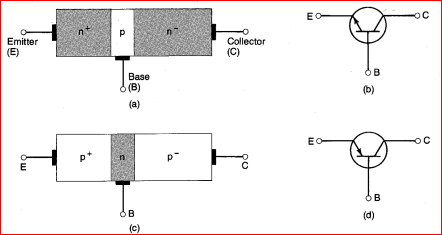
\includegraphics[width=7.5cm,height=4cm]{IMAGENES/1.PNG}
				\caption{Transistor BJT (a) NPN y (b) su símbolo y (c) PNP y (d) su símbolo. \cite{1}}
				\label{f_1}
			\end{figure}
		\end{block}
	\end{frame}
	
	\begin{frame}
		\begin{block}{Transistores CMOS}
			La tecnología CMOS hace uso de básicamente de transistores de efecto de campo NMOS y PMOS, este tipo de ciencia es más rapida y consumo menos potencia de energía que requiere otras familias. Debido a que presenta mayor densidad de integración.  
			\begin{figure}[!h]
				\centering
				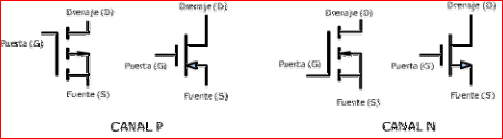
\includegraphics[width=7.5cm,height=4cm]{IMAGENES/2.PNG}
				\caption{Símbolos más comunes de los transistores PMOS y NMOS \cite{2}}
				\label{f_2}
			\end{figure}
		\end{block}
	\end{frame}
	
	\begin{frame}
		Las diferencias que presentan las familias de los CMOS y los TTLs son:
		\begin{itemize}
			\item Los CMOS presenta un mayor intervalo de voltaje y un factor de carga más elevado que los TTL.
			\item Los CMOS tienen una mayor inmunidad al ruido que los TTL.
			\item Los CMOS son más lentos en cuanto a velocidad de operación que los TTL.
			\item Los circuitos integrados CMOS es de menor consumo de potencia que los TTL.
			\item La inmunidad al ruido de CMOS es mucho mejor que los circuitos TTL.
		\end{itemize}
	\end{frame}
	
	\section{Nuevas tecnologías}
	\begin{frame}
		A lo largo de los años se empezaron a realizar estudios en los nanotubos de carbono (CNT) que presenta diferentes configuraciones, en especial en las nanométricas que están empezando a tener lugar importante en los amplificadores diferenciales, amplificadores operacionales entre otros derivados que son empleados en las tecnologías conocidas, así como en las telecomunicaciones.\\
		
		Las CNT se comportan como sistemas unidimensionales (1D) ya que sus dimensiones se encuentran en escalas nanométricas, que definen sus propiedades físicas especiales que presenta, cuyo parámetros eléctricos y ópticos son muy superiores a los semiconductores Si, Ge y GaAs.\\
		
		En la búsqueda de dispositivos cada vez más pequeños con bajo consumo de energía y alta velocidad, en ese sentido se vio como opción los derivados de los nanotubos de carbono, SWCNT (Nanotubos de carbono de pared simple) que presentan un comportamiento metálico o semiconductor que nos permite proyectae buenos hilos conductores y uniones P-N a escala nanométrica.
	\end{frame} 
	
	\subsection{Nanotransistores basados en CNT}
	\begin{frame}
		Los transistores FET estan compuestos de dos electrodos metálicos (fuente y drenaje) conectados por un semiconductor. Al variar la anchura del canal, la tensión de polarización en el electrodo llamado "puerta" controla el flujo de corriente entre la fuente y drenaje.\\
		
		En \cite{3} menciona que se demostró que los CNT se podian utilizarse en los diseños de FET. Donde los nanotubos de carbono se encuentra la parte superior, interconectando asi los dos electrodos de metales nobles.
		\begin{figure}[!ht] 
			\centering
			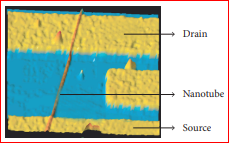
\includegraphics[width=0.25\textwidth]{IMAGENES/3.PNG}
			\caption{Imagen de transistor de efecto de campo con CNT obtenida por microscopio de fuerza atómica  \cite{3}}
			\label{f_3}
		\end{figure}
		
		
	\end{frame}
	
	\begin{frame}{Bibliografía}
		\bibliographystyle{ieeetr}
		\bibliography{bibliografia}
	\end{frame}
	
\end{document} 
